\documentclass[11pt,a4paper,onecolumn]{article} 

\usepackage[brazilian]{babel}
\usepackage[utf8]{inputenc}
\usepackage{listings}
\usepackage{color}
\usepackage{xcolor}
\usepackage{fullpage}
\usepackage{indentfirst}
\usepackage{graphicx}

\title{Relatório do Capítulo 04 de\\Introdução à Programação Paralela}
\author{Lucas Sousa de Oliveira (10/59491)}
\date{\today}

\lstdefinestyle{cc}{
  belowcaptionskip=1\baselineskip,
  breaklines=true,
  frame=l,
  xleftmargin=\parindent,
  language=C,
  showstringspaces=false,
  basicstyle=\footnotesize\ttfamily,
  keywordstyle=\bfseries\color{green!40!black},
  commentstyle=\itshape\color{purple!40!black},
  identifierstyle=\color{blue!50!black},
  stringstyle=\color{orange},
  numbers=left,
  stepnumber=1,
}
\lstdefinestyle{cbash}{
  breaklines=true,
  frame=l,
  language=bash,
  basicstyle=\footnotesize\ttfamily\color{orange},
  numbers=none,
  stepnumber=1,
  rulecolor=\color{black},
  belowcaptionskip=1\baselineskip,
  xleftmargin=\parindent,
}

\begin{document}
\maketitle

\section{Título do Capítulo}
\textit{An Application: Numerical Integration}

\section{Objetivo}
Familiarizar o aluno com a biblioteca MPI através da utilização de métodos númericos de integração para calcular a integral definida de uma função arbitrária.

\section{Resumo}
\label{sec:resumo}
Para o desenvolvimento deste capítulo, nenhum novo comando precisou ser apresentado.
Ainda assim, a metodologia de típica de escrita de um programa paralelo foi usada.
Esta metologia inclui:
\begin{enumerate}
\item Construir um programa serial para resolver um problema.
Neste caso o problema estudado foi a regra trapezoidal para a estimação de uma integral definida.
\item De forma a paralelizar o algoritmo serial, simplesmente particiona-se o conjunto de dados entre os processor.
No caso apresentado, cada processo integrou a função sobre parte do intervalo desejado.
\item Os cálculos locais produzidos pelos processos individuais são combinados para produzir o resultado final.
Aqui, cada processo enviou os resultados da sua integração para o processo 0, que somou tudo e imprimiu o resultado.
\end{enumerate}

Note que separar as variáveis pelo seu escopo, i.e. globais, aquelas com importância para todos os processos, e locais, aquelas com importância apenas para cada processo individualmente, é uma pratica importante.
Outro ponto que deve ser considerado fortemente é o comportamento imprevisível de funções de entrada e saída.
Para programas paralelos, estas funções podem ou não interagir com o terminal de qualquer máquina que estiver executando os processos, potencialmente gerando bloqueios.
Uma solução para tal problema é construir o programa de tal forma que apenas o processo 0 possa executar uma função de E/S.

\section{Exercícios}
\subsection{Escreva a primeira versão do programa de cálculo paralelizado da regra trapezoidal. Defina $\mathbf{f(x)}$ como uma função cuja integral pode ser facilmente calculada a mão, e.g. $\mathbf{f(x) = x^2}$. Compile e rode o programa para diferentes números de processos. O que acontece se o programa for rodado em apenas um processo?}
A primeira versão do programa é a apresentada abaixo.
\begin{lstlisting}[style=cc]
#include <stdio.h>
#include "mpi.h"

int main(int argc, char** argv) {
    int         my_rank;
    int         p;
    float       a = 0.0;
    float       b = 1.0;
    int         n = 1024;
    float       h;
    float       local_a;
    float       local_b;
    int         local_n;
    float       integral;
    float       total;
    int         source;
    int         dest = 0;
    int         tag = 0;
    MPI_Status  status;

    float Trap(float local_a, float local_b, int local_n, float h);
    
    MPI_Init(&argc, &argv);
    MPI_Comm_rank(MPI_COMM_WORLD, &my_rank);
    MPI_Comm_size(MPI_COMM_WORLD, &p);

    h = (b-a)/n;
    local_n = n/p;
    
    local_a = a + my_rank*local_n*h;
    local_b = local_a + local_n*h;
    integral = Trap(local_a, local_b, local_n, h);

    if (my_rank == 0) {
        total = integral;
        for (source = 1; source < p; source++) {
            MPI_Recv(&integral, 1, MPI_FLOAT, source, tag, MPI_COMM_WORLD, &status);
            total = total + integral;
        }
    } else {  
        MPI_Send(&integral, 1, MPI_FLOAT, dest, tag, MPI_COMM_WORLD);
    }

    if (my_rank == 0) {
        printf("With n = %d trapezoids, our estimate\n", n);
        printf("of the integral from %f to %f = %f\n", a, b, total);
    }

    MPI_Finalize();
}

float Trap(float local_a, float local_b, int local_n, float h) {
    float integral;
    float x;
    int i;

    float f(float x); 
    
    integral = (f(local_a) + f(local_b))/2.0;
    x = local_a;
    for (i = 1; i <= local_n-1; i++) {
        x = x + h;
        integral = integral + f(x);
    }
    integral = integral*h;
    return integral;
} 

float f(float x) {
    float return_val;
    return_val = x*x;
    return return_val;
}
\end{lstlisting}

Note na figura \ref{fig:ex1} que quando o programa é executado com um número de processos igual a $2^n$, sua integral é exata.
Isto acontece devido ao cálculo simplificado da divisão de dados.
A única diferença notável quando o programa é rodado com apenas um processo é a velocidade de computação mais elevada, uma vez que o \textit{overhead} de comunicação foi eliminado.

\begin{figure}[h!]
  \centering
  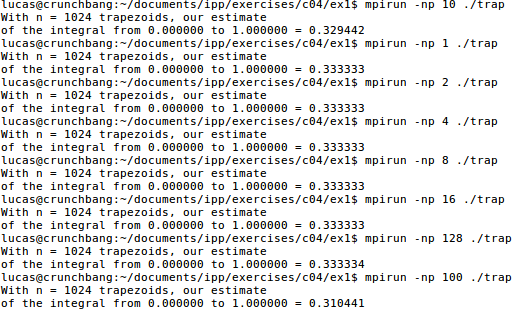
\includegraphics[width=0.9\textwidth]{../ex1/SaidaEx1}
  \caption{Resultado do teste para diversas quantidades de processos.}
  \label{fig:ex1}
\end{figure}

\subsection{Modifique o programa anterior de forma que $\mathbf{a}$, $\mathbf{b}$ e $\mathbf{c}$ sejam lidos e distribuídos pelo processo 0 - use a função Get\_data. Onde a função Get\_data deve ser colocada? Seriam necessárias outras modificações para permitir que o programa funcione, além das relacionadas com Get\_data?}
Podemos modificar o código (apresentado no final da seção \ref{sec:resumo}) da forma solicitada como está apresentado abaixo. 
\begin{lstlisting}[style=cc]
#include <stdio.h>
#include "mpi.h"

main(int argc, char** argv) {
    int         my_rank;
    int         p;
    float       a; 
    float       b;
    int         n; 
    float       h;
    float       local_a;
    float       local_b;
    int         local_n;
    float       integral;
    float       total;
    int         source;
    int         dest = 0;
    int         tag = 0;
    MPI_Status  status;

    void Get_data(float* a_ptr, float* b_ptr, int* n_ptr, int my_rank, int p);
    float Trap(float local_a, float local_b, int local_n, float h);
    
    MPI_Init(&argc, &argv);
    MPI_Comm_rank(MPI_COMM_WORLD, &my_rank);
    MPI_Comm_size(MPI_COMM_WORLD, &p);

    Get_data(&a, &b, &n, my_rank, p);

    h = (b-a)/n;
    local_n = n/p;

    local_a = a + my_rank*local_n*h;
    local_b = local_a + local_n*h;
    integral = Trap(local_a, local_b, local_n, h);

    if (my_rank == 0) {
        total = integral;
        for (source = 1; source < p; source++) {
            MPI_Recv(&integral, 1, MPI_FLOAT, source, tag, MPI_COMM_WORLD, &status);
            total = total + integral;
        }
    } else {   
        MPI_Send(&integral, 1, MPI_FLOAT, dest, tag, MPI_COMM_WORLD);
    }

    if (my_rank == 0) {
        printf("With n = %d trapezoids, our estimate\n", n);
        printf("of the integral from %f to %f = %f\n", a, b, total); 
    }

    MPI_Finalize();
}

void Get_data(float* a_ptr, float* b_ptr, int* n_ptr, int my_rank, int p) {

    int source = 0;
    int dest;
    int tag;
    MPI_Status status;

    if (my_rank == 0){
        printf("Enter a, b, and n\n");
        scanf("%f %f %d", a_ptr, b_ptr, n_ptr);
        for (dest = 1; dest < p; dest++){
            tag = 0;
            MPI_Send(a_ptr, 1, MPI_FLOAT, dest, tag, MPI_COMM_WORLD);
            tag = 1;
            MPI_Send(b_ptr, 1, MPI_FLOAT, dest, tag, MPI_COMM_WORLD);
            tag = 2;
            MPI_Send(n_ptr, 1, MPI_INT, dest, tag, MPI_COMM_WORLD);
        }
    } else {
        tag = 0;
        MPI_Recv(a_ptr, 1, MPI_FLOAT, source, tag, MPI_COMM_WORLD, &status);
        tag = 1;
        MPI_Recv(b_ptr, 1, MPI_FLOAT, source, tag, MPI_COMM_WORLD, &status);
        tag = 2;
        MPI_Recv(n_ptr, 1, MPI_INT, source, tag, MPI_COMM_WORLD, &status);
    }
}

float Trap(float local_a, float local_b, int local_n, float h) {
    float integral;
    float x; 
    int i; 

    float f(float x);

    integral = (f(local_a) + f(local_b))/2.0; 
    x = local_a; 
    for (i = 1; i <= local_n-1; i++) { 
        x = x + h; 
        integral = integral + f(x); 
    } 
    integral = integral*h; 
    return integral;
}

float f(float x) { 
    float return_val; 
    return_val = x*x;
    return return_val; 
}
\end{lstlisting}

Note que nenhuma outra modificação foi necessária, apesar de se ter utilizado a função \textit{Trap} auxiliar para isolar o \textit{loop} de cálculo.

\begin{figure}[h!]
  \centering
  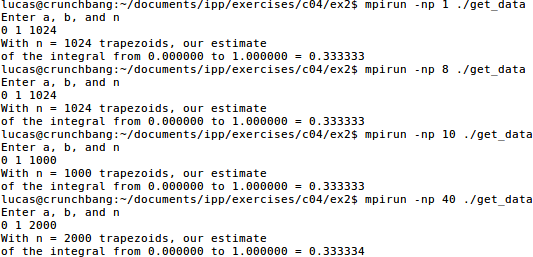
\includegraphics[width=0.9\textwidth]{../ex2/SaidaEx2}
  \caption{Resultado ao se usar diversos números de processos e intervalos.}
  \label{fig:ex2}
\end{figure}

\section{Trabalho de programação}
\subsection{Modifique o programa paralelo com a regra trapezoidal de forma que diversas funções possam ser escolhidas e passadas para a função \textit{Trap}. Apresente ao usuário uma menu de funções possíveis.}

O código com as devidas modificações está mostrado abaixo. A saída do programa está na figura \ref{fig:exp}.
\begin{lstlisting}[style=cc]
#include <stdio.h>
#include "mpi.h"

main(int argc, char** argv) {
    int         my_rank;   
    int         p;         
    float       a;         
    float       b;         
    int         n;         
    int         f;         
    float       h;         
    float       local_a;   
    float       local_b;   
    int         local_n;   
                           
    float     (*local_f)(float); 
    float       integral;  
    float       total;     
    int         source;    
    int         dest = 0;  
    int         tag = 0;
    MPI_Status  status;

    void Get_data(float* a_ptr, float* b_ptr, int* n_ptr, int* f_ptr, int my_rank, int p);
    float Trap(float local_a, float local_b, int local_n, float (*f)(float), float h);    

    
    MPI_Init(&argc, &argv);
    MPI_Comm_rank(MPI_COMM_WORLD, &my_rank);
    MPI_Comm_size(MPI_COMM_WORLD, &p);

    Get_data(&a, &b, &n, &f, my_rank, p);

    float k(float);
    float l(float);
    float m(float);

    switch(f){
        case 0: local_f = k;break;
        case 1: local_f = l;break;
        case 2:
       default: local_f = m;break;
    }

    h = (b-a)/n;    
    local_n = n/p;  


    local_a = a + my_rank*local_n*h;
    local_b = local_a + local_n*h;
    integral = Trap(local_a, local_b, local_n,local_f, h);

    if (my_rank == 0) {
        total = integral;
        for (source = 1; source < p; source++) {
            MPI_Recv(&integral, 1, MPI_FLOAT, source, tag, MPI_COMM_WORLD, &status);
            total = total + integral;
        }
    } else {   
        MPI_Send(&integral, 1, MPI_FLOAT, dest, tag, MPI_COMM_WORLD);
    }

    
    if (my_rank == 0) {
        printf("With n = %d trapezoids, our estimate\n", n);
        printf("of the integral from %f to %f = %f\n", a, b, total); 
    }
	
	MPI_Finalize();
} 
void Get_data(float* a_ptr, float* b_ptr, int* n_ptr,int* f_ptr, int my_rank, int p) {
    int source = 0;    
    int dest;          
    int tag;
    MPI_Status status;

    if (my_rank == 0){
        printf("Functions (f):\n0. x**2\n1. x**2+1\n2. x**2+2\n")
        printf("Enter a, b, n, and f\n");
        scanf("%f %f %d %d", a_ptr, b_ptr, n_ptr, f_ptr);
        for (dest = 1; dest < p; dest++){
            tag = 0;
            MPI_Send(a_ptr, 1, MPI_FLOAT, dest, tag, MPI_COMM_WORLD);
            tag = 1;
            MPI_Send(b_ptr, 1, MPI_FLOAT, dest, tag, MPI_COMM_WORLD);
            tag = 2;
            MPI_Send(n_ptr, 1, MPI_INT, dest, tag, MPI_COMM_WORLD);
            tag = 3;
            MPI_Send(f_ptr, 1, MPI_INT, dest, tag, MPI_COMM_WORLD);
        }
    } else {
        tag = 0;
        MPI_Recv(a_ptr, 1, MPI_FLOAT, source, tag, MPI_COMM_WORLD, &status);
        tag = 1;
        MPI_Recv(b_ptr, 1, MPI_FLOAT, source, tag, MPI_COMM_WORLD, &status);
        tag = 2;
        MPI_Recv(n_ptr, 1, MPI_INT, source, tag, MPI_COMM_WORLD, &status);
        tag = 3;
        MPI_Recv(f_ptr, 1, MPI_INT, source, tag, MPI_COMM_WORLD, &status);
    }
}
float Trap(float local_a, float local_b, int local_n, float (*local_f)(float), float h) { 
    float integral;    
    float x; 
    int i;

    integral = ((*local_f)(local_a) + (*local_f)(local_b))/2.0; 
    x = local_a; 
    for (i = 1; i <= local_n-1; i++) { 
        x = x + h; 
        integral = integral + (*local_f)(x); 
    } 
    integral = integral*h; 
    return integral;
} 
float k(float x) { 
    float return_val; 
    
     
    return_val = x*x;
    return return_val; 
} 
float l(float x) { 
    float return_val; 
    return_val = x*x+1;
    return return_val; 
} 
float m(float x) { 
    float return_val; 
    return_val = x*x+2;
    return return_val; 
}
\end{lstlisting}

Note que cada processo deve primeiro enviar a mensagem para depois esperar, uma vez que se o contrário for feito, todos os processos esperarão indefinidamente uns pelos outros, o que caracteriza um \textit{deadlock}.

\begin{figure}[h!]
  \centering
  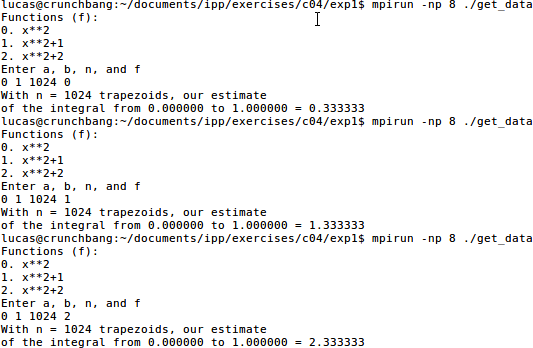
\includegraphics[width=0.9\textwidth]{../exp1/SaidaExp1}
  \caption{Resultado do programa modificado.}
  \label{fig:exp}
\end{figure}

\subsection{Uma alternativa mais precisa que a regra trapezoidal é a regra de Simpson.
A idéia básica é de aproximar a curva de $\mathbf{f(x)}$ por arcos de parabolas ao invés de segmentos de linhas.
Suponha que $\mathbf{p < q}$ são números reais, e suponha que $\mathbf{r}$ é o ponto médio do segmento $\mathbf{\left[p,q\right]}$.
Se nós fizermos $\mathbf{h = (q-p)/2}$, então a equação da parábola passando pelos pontos $\mathbf{(p,f(p))}$,$\mathbf{(r,f(r))}$ e $\mathbf{(q,f(q))}$ é:
$$\mathbf{y = \frac{f(p)}{2h^2}(x-r)(x-q)-\frac{f(r)}{h^2}(x-p)(x-q)+\frac{f(q)}{2h^2}(x-p)(x-r)}.$$
Se integrarmos esta forma de $\mathbf{p}$ a $\mathbf{q}$, teremos $$\mathbf{\frac{h}{3}[f(p)+4f(r)+f(q)]}.$$
Assim, se usarmos a mesma notação que usamos na discussão da regra trapezoidal e assumirmos que $\mathbf{n}$, o número de subintervalos de $\mathbf{[a,b]}$, é par, podemos aproximar
$$\mathbf{\int_{a}^{b}f(x)dx = \frac{h}{3}[f(x_0)+4f(x_1)+2f(x_2)+\cdots+2f(x_{n-2})+4f(x_{n-1})+f(x_n)]}.$$
Assumindo que $\mathbf{n/p}$ é par, escreva:}
\subsubsection*{a. um programa serial que use a regra de Simpson para estimar $\mathbf{\int_{a}^{b}f(x)dx}$.}
\begin{lstlisting}[style=cc]
#include <stdio.h>

main() {
    float  integral;
    float  a, b;
    int    n;
    float  h;
    float  x;
    int    i;

    float f(float x);

    printf("Enter a, b, and n\n");
    scanf("%f %f %d", &a, &b, &n);

    h = (b-a)/n;
    integral = (f(a) + f(b));
    x = a;
    for (i = 1; i <= n-1; i++) {
        x = x + h;
        integral = integral + (i%2?4:2)*f(x);
    }
    integral = integral*h/3.0;

    printf("With n = %d trapezoids, our estimate\n", n);
    printf("of the integral from %f to %f = %f\n", a, b, integral);
}

float f(float x) {
    float return_val;
    return_val = x*x;
    return return_val;
}
\end{lstlisting}

\subsubsection*{b. um programa paralelo que use a regra de Simpson para estimar $\mathbf{\int_{a}^{b}f(x)dx}$.}
\begin{lstlisting}[style=cc]
#include <stdio.h>
#include "mpi.h"

main(int argc, char** argv) {
    int         my_rank;
    int         p;
    float       a;
    float       b;
    int         n;
    int         f;
    float       h;
    float       local_a;
    float       local_b;
    int         local_n;
    float     (*local_f)(float);
    float       integral;
    float       total;
    int         source;
    int         dest = 0;
    int         tag = 0;
    MPI_Status  status;

    void Get_data(float* a_ptr, float* b_ptr, int* n_ptr, int* f_ptr, int my_rank, int p);
    float Trap(float local_a, float local_b, int local_n, float (*f)(float), float h);

    MPI_Init(&argc, &argv);
    MPI_Comm_rank(MPI_COMM_WORLD, &my_rank);
    MPI_Comm_size(MPI_COMM_WORLD, &p);

    Get_data(&a, &b, &n, &f, my_rank, p);

    float k(float);
    float l(float);
    float m(float);

    switch(f){
        case 0: local_f = k;break;
        case 1: local_f = l;break;
        case 2:
       default: local_f = m;break;
    }

    h = (b-a)/n;
    local_n = n/p;

    local_a = a + my_rank*local_n*h;
    local_b = local_a + local_n*h;
    integral = Trap(local_a, local_b, local_n,local_f, h);

    if (my_rank == 0) {
        total = integral;
        for (source = 1; source < p; source++) {
            MPI_Recv(&integral, 1, MPI_FLOAT, source, tag, MPI_COMM_WORLD, &status);
            total = total + integral;
        }
    } else {   
        MPI_Send(&integral, 1, MPI_FLOAT, dest, tag, MPI_COMM_WORLD);
    }

    if (my_rank == 0) {
        printf("With n = %d trapezoids, our estimate\n", n);
        printf("of the integral from %f to %f = %f\n", a, b, total); 
    }

    MPI_Finalize();
}

void Get_data(
         float*  a_ptr, 
         float*  b_ptr, 
         int*    n_ptr,
         int*    f_ptr,
         int     my_rank, 
         int     p) {

    int source = 0;
    int dest;
    int tag;
    MPI_Status status;

    if (my_rank == 0){
        printf("Enter a, b, n, and f\n");
        scanf("%f %f %d %d", a_ptr, b_ptr, n_ptr, f_ptr);
        for (dest = 1; dest < p; dest++){
            tag = 0;
            MPI_Send(a_ptr, 1, MPI_FLOAT, dest, tag, MPI_COMM_WORLD);
            tag = 1;
            MPI_Send(b_ptr, 1, MPI_FLOAT, dest, tag, MPI_COMM_WORLD);
            tag = 2;
            MPI_Send(n_ptr, 1, MPI_INT, dest, tag, MPI_COMM_WORLD);
            tag = 3;
            MPI_Send(f_ptr, 1, MPI_INT, dest, tag, MPI_COMM_WORLD);
        }
    } else {
        tag = 0;
        MPI_Recv(a_ptr, 1, MPI_FLOAT, source, tag, MPI_COMM_WORLD, &status);
        tag = 1;
        MPI_Recv(b_ptr, 1, MPI_FLOAT, source, tag, MPI_COMM_WORLD, &status);
        tag = 2;
        MPI_Recv(n_ptr, 1, MPI_INT, source, tag, MPI_COMM_WORLD, &status);
        tag = 3;
        MPI_Recv(f_ptr, 1, MPI_INT, source, tag, MPI_COMM_WORLD, &status);
    }
}

float Trap(
          float  local_a, 
          float  local_b, 
          int    local_n,
          float  (*local_f)(float),
          float  h
        ) { 

    float integral;
    float x; 
    int i;

    integral = ((*local_f)(local_a) + (*local_f)(local_b)); 
    x = local_a; 
    for (i = 1; i <= local_n-1; i++) { 
        x = x + h; 
        integral = integral + (i%2?4:2)*(*local_f)(x); 
    } 
    integral = integral*h/3.0; 
    return integral;
}
float k(float x) { 
    float return_val;
    return_val = x*x;
    return return_val; 
}
float l(float x) { 
    float return_val; 
    return_val = x*x+1;
    return return_val; 
}
float m(float x) { 
    float return_val; 
    return_val = x*x+2;
    return return_val; 
}
\end{lstlisting}

\section{Conclusão}
Conclui-se que a biblioteca MPI permite a distribuição de processamento entre diversos computadores, podendo assim aumentar o poder computacional diponível para um programa.
As ferramentas apresentadas aqui se mostraram extremamente úteis, apesar de simples, para as tarefas de computaçao paralela e distribuída.

\section{Referências}
\paragraph{Pacheco, P.S.,} (1997) \textit{Parallel Programming with MPI}. Morgan Kaufmann.

\end{document}
